\chapter{Literature study}
This thesis is about the training of neural networks as a feasibility problem, this approach is based on the works of \citet{elser2019learning} and \citet{bergmeister2025projection}. A comprehensive literature study is provided below, its structured into 4 main categories.
\begin{itemize}
    \item Motivation for alternatives to gradient-based optimization in deep learning.
    \item The relevant constraints in an feasibility based neural network.
    \item the projections necessary to implement these constraints.
    \item Methods to solve feasibility problems for non convex sets.
\end{itemize}
\subsection{Constraints neural network}
There are 2 main methods of modeling the network presented in the literature \citet{elser2019learning} proposes a neuron based approach in which constraints are modeled for each output neuron, \cite{bergmeister2025projection} on the other hand proposes to use primitive functions as a building block. To elaborate the constraints on the following network is modeled.
\begin{figure}[h!]
  \centering
    \begin{tikzpicture}[
    x=2.0cm, y=1.2cm,
    neuron/.style={circle, draw, minimum size=7mm, inner sep=1pt, font=\small},
    activation/.style={rectangle, draw, minimum size=5mm, font=\scriptsize, rounded corners=2pt, fill=gray!10},
    >=Stealth,
    weight/.style={font=\scriptsize, midway, sloped}
  ]

  % Input layer (3 inputs + bias)
  \node[neuron] (I1) at (0, 1) {$x_1$};
  \node[neuron] (I2) at (0, 0) {$x_2$};
  \node[neuron] (I3) at (0,-1) {$x_3$};
  \node[neuron] (B)  at (0, 2) {$1$}; % bias

  % Hidden layer (pre-activation)
  \node[neuron] (H1) at (2, 1) {$h_1$};
  \node[neuron] (H2) at (2, 0) {$h_2$};
  \node[neuron] (H3) at (2,-1) {$h_3$};

  % Activation layer
  \node[activation, right=0.8cm of H1] (A1) {$f(h_1)$};
  \node[activation, right=0.8cm of H2] (A2) {$f(h_2)$};
  \node[activation, right=0.8cm of H3] (A3) {$f(h_3)$};

  % Post-activation "x" layer
  \node[neuron, right=0.8cm of A1] (X1) {$x_1^{(2)}$};
  \node[neuron, right=0.8cm of A2] (X2) {$x_2^{(2)}$};
  \node[neuron, right=0.8cm of A3] (X3) {$x_3^{(2)}$};

  % Output layer (single output)
  \node[neuron, right=0.8cm of X2] (O) {$y$};

  % Input -> hidden
  \foreach \i in {1,2,3} {
    \foreach \j in {1,2,3} {
      \draw[->] (I\i) -- (H\j);
    }
  }

  % Bias -> hidden
  \foreach \j in {1,2,3} {
    \draw[->] (B) -- (H\j);
  }

  % Hidden -> activation
  \foreach \j in {1,2,3} {
    \draw[->] (H\j) -- (A\j);
  }

  % Activation -> post-activation x layer
  \foreach \j in {1,2,3} {
    \draw[->] (A\j) -- (X\j);
  }

  % Post-activation x layer -> output
  \foreach \j in {1,2,3} {
    \draw[->] (X\j) -- (O);
  }

  % Add weight labels only for paths involving h1
  \draw[->] (I1) -- node[weight, above] {$w_{h_1,x_1}^{(1)}$} (H1);
  \draw[->] (I2) -- node[weight, above] {$w_{h_1,x_2}^{(1)}$} (H1);
  \draw[->] (I3) -- node[weight, above] {$w_{h_1,x_3}^{(1)}$} (H1);
  \draw[->] (B)  -- node[weight, above] {$b_{h_1}^{(1)}$} (H1);
  \draw[->] (X1) -- node[weight, above] {$w_{y,x_1^{(2)}}^{(2)}$} (O);

  % Layer labels
  \node[above,font=\small] at (0,2.3) {Input layer};
  \node[above,font=\small] at (5,0.8) {Output layer};

\end{tikzpicture}
 
    \caption{demo network that will be used to show how constraints are modeled}
    \label{fig:demo-network}
\end{figure}
\subsubsection{Neuron based approach}
\includecomment{TODO add proper indicess}
The constraints on the neuron $h_1$ are the following:
The subscript denotes the neuron, the superscript denotes the sample of the batch 
\begin{itemize}
    \item $\forall k: h_1^k = h_1$ its has the same value for all of the samples in the batch.
    \item  $\forall k, j: w_{h_1x_j}^k = w_{h_1x_j}$ Weights are the same for all items in a batch
    \item  $\sum{w_{h_1x_j}^2} = \sigma^2$ weights are normalized
    \item $\sum{w_{h_1x_j}x_j} + w_{h_1,b_1}b_1=h_1$ output of $h_1$ is a linear combination of input variables 
    \item $f(h_1) = x_1^{(2)}$ the input of the next layer is equal to the activation function applied to $h_1$
\end{itemize}
The constraints for input / output nodes are slightly different as they need to be constrained to the input / output value.
This adds the following constraints:
\begin{itemize}
    \item  $\forall k: x_1^k = d_1^k$ the input node matches the input data value.
\end{itemize}
\begin{figure}
    \centering
    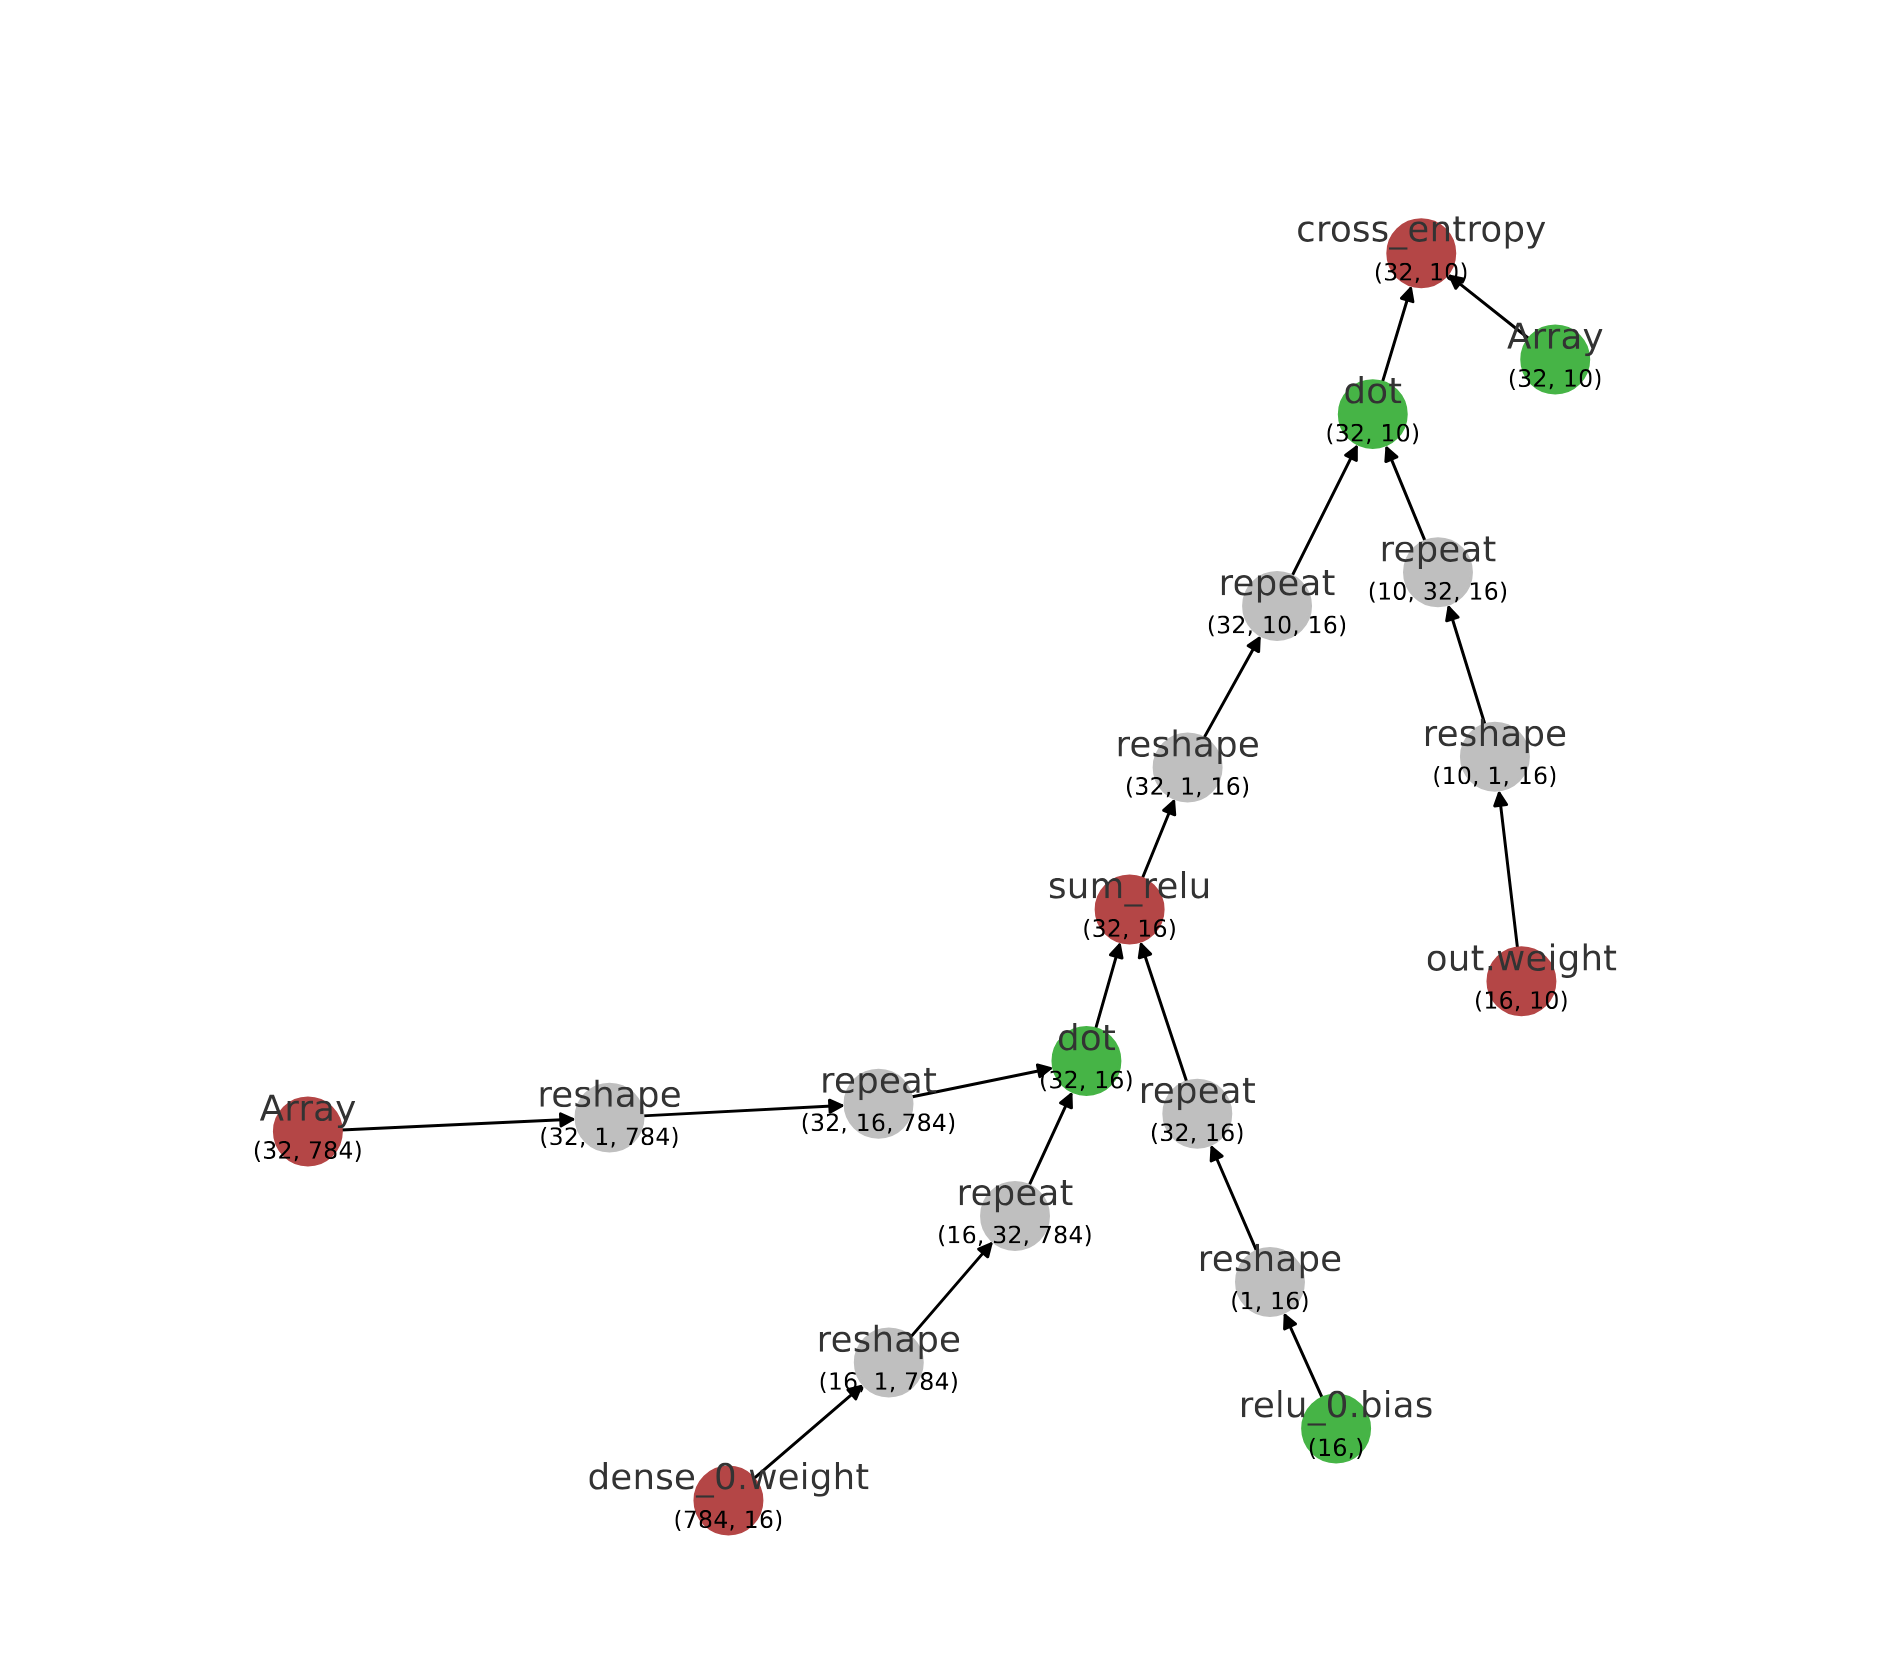
\includegraphics[width=0.5\linewidth]{images/computational graph.png}
    \caption{van papaer1}
    \label{fig:placeholder}
\end{figure}
\subsubsection{computational graph approach}
Given the input x, loss function f and output y; we can build a computational graph where the nodes represent either constant inputs, parameters of the model, operation of a vector to scalar function f. Each edge represents that the output of node u serves as input to node. The paper suggests that we can get tractable projection operators if we only use scalar values on the edges.\\
For each node in the network a set of constraints on its edge value's is made. For example the constraint for an constant node is that the outgoing edge has the same value as the node. For parameter nodes a constraint is added that all outgoing edges must have the same value. \\
For some specefics nodes, other constraints are added ass well, for example the dot node, has the constraint that the dot product of its input has to equeal its output value,.... \\
\subsubsection{Implementation of conv2d}
Convolutional neural networks, are a problem in this framework because of their excessive memory usage. The implementation works as follows, first a set of patches is generated, afterwards a linear layer is computed. And afterwards the parameters are updated as if this was the computation on a batch of data
\newpage
\subsection{projections}
The following section is all based on Projections and monotone operators by bauschke.
To find a feasible solution given these constraints, projections onto the set of possible solutions given the constraints are used. As both approaches use roughly the same constraints, a derivations of their projection is provided
\subsubsection{definition + basic properties}\ref{bauschkyProjections}
To introduce projections, first the distance from an element $a$ from a set X to a subset of X named C needs to be defined.
$d(a,C) := inf_{a'\in C}(||a-a'||)$.
Subsequently the projection is defined as the point in the subset C that minimizes this distance. Denoted as $P_C(a)$.
Next I am going to go over some of the most important properties of this operator.
A coupe of important properties of this operator, given that C is closed and convex are the following:
(This is straight copy from baushky \ref{bauschkyProjections})\\
Suppose \(C\) is a closed convex nonempty subset of \(X\) and \(x \in X\). Then:

\begin{enumerate}[(i)]
    \item \textbf{(translation)}  
    \[
        P_{z + C}(x) = z + P_C(x - z), \qquad \forall z \in X .
    \]

    \item \textbf{(dilation)}  
    \[
        P_{rC}(x) = r \, P_C\!\left(\frac{x}{r}\right), \qquad \forall r \neq 0 .
    \]
doc
\end{enumerate}

% \\bullshit-->
% 1) Geometric interpretation ( if C is closed and convex):
% the projection happens perpendicular onto the set, $z-P_C(a) \in \partial \iota_{C}(P_C(a))$. in this case $\partial \iota_{C}(P_C(a))$ is equal to the normal cone to C meaning that 
% <-- bullshit
(Assuming C is Convex and closed)
A very important property for our purposes is that every projection is 
\emph{firmly nonexpansive}, and therefore \(1\)-attracting. 
Using this fact, we obtain the following result.

Assume that
\[
    C = \bigcap_{i=1}^n C_i
\]
and that the intersection is nonempty. Then the fixed-point set of the 
weighted average of the projections satisfies
\[
    \operatorname{Fix}\!\left(\sum_{i=1}^n \omega_i P_i\right) = C,
\]
where each weight \(\omega_i > 0\) and 
\(\sum_{i=1}^n \omega_i = 1\).


\begin{itemize} 
    \item \textbf{bilinear constraint}
    \begin{itemize}
    \item  \textbf{motivation}:
    As we run in to serious memory limitations when trying to calculate the conv2d using the method implemented in pjax an alternative method was developed. By first calculating the fft and padding, and performing the hadamar product, and then reversing the operation we have a more memory efficient implement ion of the convolution. But this requires a new projection to be calculate, this one is presented below
    
    \item \textbf{definition}:\\
    $Y\in\mathbb{C}^{n,n} \in \mathbb{C}, X\in\mathbb{C}^{n,n}, W \in  \mathbb{C}^{n,n}$
     We try to satisfy the following constraints
    \begin{equation}
        \begin{split}
            & y'=w' \circ x'\\
            &\min( ||x-x'||^2_F + ||w-w'||^2_F+||y-y'||^2_F)
        \end{split}
    \end{equation}
    \[
    y = w \circ x, 
    \qquad w, x, y \in \mathbb{C}.
    \]
    
    Let 
    \[
    w = w_r + i w_i, \qquad x = x_r + i x_i.
    \]
    
    Then the Hadamard product (elementwise product) is just complex multiplication:
    
    \[
    y = wx 
      = (w_r + i w_i)(x_r + i x_i).
    \]
    
    Expanding:
    
    \[
    y 
    = (w_r x_r - w_i x_i)
      + i(w_r x_i + w_i x_r).
    \]
    
    Thus
    
    \[
    \boxed{
    \begin{aligned}
    y_r &= w_r x_r - w_i x_i, \\
    y_i &= w_r x_i + w_i x_r.
    \end{aligned}}
    \]
    
    As we still want our solution to be as close to the original solution as possible, 
    Given a new  value
    
    \[
    \|y - y'\|^2
    = (y_r - y_r')^2 + (y_i - y_i')^2.
    \]
    \[
    \|x - x'\|^2
    = (x_r - x_r')^2 + (x_i - x_i')^2.
    \]
    \[
    \|w -w'\|^2
    = (w_r - w_r')^2 + (w_i - w_i')^2.
    \]
    
    Constructing the Lagrangian results in the following equation
    \[
    \mathcal{L}
    = \|w -w'\|^2 + \|x - x'\|^2 + \|y - y'\|^2
    + \lambda_r \big( w_r' x_r' - w_i' x_i' - y_r',\big)
    + \lambda_i \big(w_r' x_i' + w_i' x_r' - y_i'\big).
    \]
    Taking the partial derivatives of this to zero results in the following set of equations
    \[
    \left(
    \begin{array}{c}
        2(w_r' - w_r) + \lambda_i x_i' + \lambda_r x_r' \\[6pt]
        2(w_i' - w_i) - \lambda_r x_i' + \lambda_i x_r' \\[6pt]
        2(x_r' - x_r) + \lambda_i w_i' + \lambda_r w_r' \\[6pt]
        2(x_i' - x_i) - \lambda_r w_i' + \lambda_i w_r' \\[6pt]
        2(y_r' - y_r) - \lambda_r \\[6pt]
        2(y_i' - y_i) - \lambda_i \\[6pt]
        w_r' x_r' - w_i' x_i' - y_r' \\[6pt]
        w_r' x_i' + w_i' x_r' - y_i'
    \end{array}
    \right)
    \]   
    Taking the partial derivatives with respect to real and imaginary components yields a large $8 \times 8$ system. However, we can significantly accelerate the solution by grouping these terms into complex variables. Let $L = (\lambda_r + i\lambda_i)/2$. The stationarity conditions simplify to a compact complex form:
    
    \[
    \begin{aligned}
    w' - w + L \overline{x'} &= 0 \implies w' = w - L \overline{x'} \\
    x' - x + L \overline{w'} &= 0 \implies x' = x - L \overline{w'} \\
    y' - y - L &= 0 \implies y' = y + L
    \end{aligned}
    \]
    
    We can solve this coupled system for $w'$ and $x'$ explicitly in terms of $L$. By taking the conjugate of the expression for $x'$ and substituting it into the expression for $w'$:
    
    \[
    w' = w - L(\overline{x} - \overline{L} w') = w - L\overline{x} + |L|^2 w'
    \]
    
    Rearranging terms allows us to isolate $w'$ (and similarly $x'$):
    
    \[
    w'(1 - |L|^2) = w - L\overline{x} \implies w' = \frac{w - L\overline{x}}{1 - |L|^2}
    \]
    \[
    x' = \frac{x - L\overline{w}}{1 - |L|^2}
    \]
    
    Finally, substituting these explicit forms back into the constraint $y' = w'x'$ results in a single complex equation for $L$:
    
    \[
    \frac{(w - L\overline{x})(x - L\overline{w})}{(1 - |L|^2)^2} - (y + L) = 0
    \]
    
    This reduces the problem from solving an $8 \times 8$ real system to finding the root of a single complex equation (equivalent to a $2 \times 2$ real system), which is computationally much more efficient and memory friendly.

    
    \end{itemize}

    \item \textbf{haddamar constraint}
    \begin{itemize}
    \item \textbf{motivation}
        Find the minimal changes needed to be made to x, w and y to make it fit the current batch.
    \item \textbf{definition}:\\
    assume that y is the output, w are the weight in the layer and x is the input of the layer with
    $y \in \mathbb{R}, x\in\mathbb{R}^n, w \in  \mathbb{R}^{1*n}$
     We try to satisfy the following constraints
    \begin{equation}
        \begin{split}
            &\sigma y'=w'x'\\
            &\min( ||x-x'||^2 + ||w-w'||^2+\gamma^2*(y-y')^2)
        \end{split}
    \end{equation}
    For output layers we can assume that $\gamma$ equals infinity as we want the output of the network to equal the trainings data.
    \item \textbf{derivation projection}:\\
    derivation using Lagrange multiplier. 
    \begin{equation}
        \begin{split}
            L\left(y',x',w',\lambda\right) &= \left(||x-x'||^2 + ||w-w'||^2+\gamma^2||y-y'||^2\right) +\lambda\left(\sigma y'-w'x'\right) \\
            \nabla L\left(y',x',w',\lambda\right) &=  0=
        \begin{bmatrix}
            \sigma y'-w'x'\\
            -y' + y - \lambda\frac{\sigma}{2 \gamma^2} \\
            -x' + x + \lambda\frac{w'^\top}{2}\\
            -w' + w +\lambda\frac{x'^\top}{2}\\
        \end{bmatrix}
        \end{split}
    \end{equation}
    simplifying this using the substitution $u=\frac{\lambda}{2}$ results in 
    \begin{equation}
        \nabla L\left(y,x,w,u\right) =  0= 
       \begin{bmatrix}
            y'-y  + \frac{\sigma u}{\gamma^2})\\
            x'-x -w'^\top u\\
            w'-w - x'^\top u
        \end{bmatrix}\\
    \end{equation}
    To find the solution to this problem we set the derivative to zero.
    \begin{equation}
        \begin{split}
        w' &=w  +u\left(x + u w'^\top\right)^\top\\
        w' &= \frac{w + u x^\top}{(1-u^2)} \\        
        \end{split}
    \end{equation}
    Similar derivation for x and y results in 
    \begin{equation}
        \begin{split}
        x'&= \frac{x + u w^\top}{(1-u^2)} \\       
        y'&= y- \frac{\sigma u}{\gamma^2})\
        \end{split}
    \end{equation}
    substituting this into 1 results in 
    
    \begin{equation}
        \begin{split}
            &\sigma y'=w'x'\\
            &\sigma\left(y+ \frac{\sigma u}{\gamma^2}\right) = \left(\frac{x + u w^\top}{(1-u^2)} \right)\left(\frac{x + u w^\top}{(1-u^2)}\right)\\
            &\sigma\left(y+ \frac{\sigma u}{\gamma^2}\right) = \frac{\left(w + u x^\top\right)\left(x + u w^\top\right)}{\left(1-u^2\right)^2}\\
            &\sigma\left(y+ \frac{\sigma u}{\gamma^2}\right) =\frac{wx + u\left(ww^\top + x^\top x\right) + u^2 x^\top w^\top}{\left(1-u^2\right)^2}
        \end{split}
    \end{equation}
    simplifying this using the substitution $p=wx$ and $q=ww^\top + x^\top x$ results in 
    \begin{equation}
        \begin{split}
            &\sigma\left(y+ \frac{\sigma u}{\gamma^2}\right) = \frac{p\left(1+u^2\right) + uq}{\left(1-u^2\right)^2}\\
            &h\left(u\right) =0 = \frac{p\left(1+u^2\right) + uq}{\left(1-u^2\right)^2} - \sigma y + \frac{\sigma ^2 u}{\gamma^2}
        \end{split}
    \end{equation}
    To find the optimal value of u, newton steps are used. to do this the derivative of $h(u)$ is used.
    \begin{equation}
        u_k = u_{k-1} - \frac{h\left(u\right)}{ \frac{dh\left(u\right)}{du}}
    \end{equation}
    TODO:INSERT CONVERGENCE dingen
    
    
\end{itemize}


    \item \textbf{minus bilinear constraint?}\\
    what if we define $y_i$ as $|w^\top - x|^2_2$ instead of using the matrix vector product.

to find the projection onto this constraint, we obtain the following Lagrangian.
\begin{equation}
    \begin{split}
        &y'=|w'^\top - x'|^2\\
        &\min( ||x-x'||^2 + ||w-w'||^2)
    \end{split}
\end{equation}
To simplify the math, and as the result of real world testing the assumption is made that $y_0=y'$ (An early hypothesis is that this stabilizes training a bit).

This results in the following Lagrangian.
\begin{equation}
    \begin{split}
        L\left(x',w',\lambda\right) &= \left(||x-x'||^2 + ||w-w'||^2\right) +\lambda\left(y-|w' - x'|^2_2\right) \\
        \nabla L\left(y,x,w,\lambda\right) &=  0=
    \begin{bmatrix}
        y-|w' - x'|^2_2\\
        x'(\lambda -1) + x + w'\\
        w'(\lambda -1) + w + x'\\
    \end{bmatrix}
    \end{split}
\end{equation}
Reworking the equations to only be in function of $\lambda$ results in 
\begin{equation}
    \lambda = \frac{1-\sqrt{\frac{|w-x|^2_2}{y}} }{2}
\end{equation}
Sadly using this in practices results in terrible performance, the reason for this is still work in progress. 


\begin{equation}
    \begin{split}
    \begin{bmatrix}
        x'(1 - 2*\lambda) = x(1-\lambda) + w\\
        w'(1 - 2*\lambda) = w(1-\lambda) + x\\
    \end{bmatrix}
    \end{split}
\end{equation}
Subsituting both of these equations into the constraint results in the folowing formula for $\lambda$
\begin{equation}
    \lambda
\end{equation}

\begin{equation}
    \begin{split}
        L\left(x',w',\lambda\right) &= \left(||x-x'||^2 + ||w-w'||^2\right) +\lambda\left(y-|w' - x'|^2_2\right) \\
        \nabla L\left(y,x,w,\lambda\right) &=  0=
    \begin{bmatrix}
        y-|w' - x'|^2_2\\
        x'(\lambda -1) + x + w'\\
        w'(\lambda -1) + w + x'\\
    \end{bmatrix}
    \end{split}
\end{equation}



    \item \textbf{step function activation}\\
    A possible activation function is the step activation.
The formulation of the activation function is as follows:
        \begin{equation}
            f\left(x\right)=
            \begin{cases}
            0, x<=0\\
            \delta, x>=0
            \end{cases}
        \end{equation}
        and the constraint for activation functions is the following
        \begin{equation}
            y=f\left(Wx\right)
        \end{equation}
We want to find a feasible solution that changes our current parameters the least
\[
\min_{\left(x, y, w\right)} \|x - x'\|^2 + \|y - y'\|^2 + \|w - w'\|^2
\]

\[
x \in \mathbb{R}^m, \quad y \in \mathbb{R}^n, \quad w \in \mathbb{R}^{m\times n}
\]
To find a formula for feasible solutions, we use the lagragian multiplier method.

\[
L\left(x,w,y\right) = \left(x-x'\right)^\top\left(x-x'\right) + \left(y-y'\right)^\top\left(y-y'\right) + \left(w-w'\right)^\top\left(w-w'\right) + \lambda^\top\left(f\left(wx\right)-y\right)
\]
finding the optimal solution of this  system results in the following parameters.
\[
\frac{\partial L}{\partial \lambda} = 0 \quad \Rightarrow \quad f\left(wx\right) = y \quad \Rightarrow \forall i\in [0,n) \quad y_i = \begin{cases}
            \delta, W_{i,:}x>=0\\
            0, W_{i,:}x>=0
            \end{cases}
\]

\[
\frac{\partial L}{\partial x} =0 \quad \Rightarrow
2x - 2x'  = 0 \quad \Rightarrow \quad x = x'
\]

\[
\frac{\partial L}{\partial vec\left(W\right)} =0 \quad \Rightarrow
2vec\left(W\right) - 2vec\left(W'\right)  = 0 \quad \Rightarrow \quad vec\left(W\right) = vec\left(W'\right)
\]


Note on gapped step activation function, I can't figure out the math for this :/ but a cheat code for this is defining another constraint which enforces y to lie between -delta/2 and delta/2. this should result in the same end result of a more robust solver as the model is forced to make a decission.
    \item \textbf{relu activation}\\
    Another possible activation function is the relu activation.
T
The projection to relu is the solution to either of these 2 cases that has minimal changes to x and w and y.




\end{itemize}

\subsection{Solving feasability problems}
\subsubsection{What is a feasbility problem}
The problem we are trying to solve is to find a feasable point in the intersection of 2 constraint sets. Assuming A and B are sets, We try to find the point X
\begin{equation}
    x \in A \cap B
\end{equation}
To simplify the notation for the upcoming section we define the projection onto a set as 
\begin{equation}
\mathbb{P}_C(x) := \left\{ z \in C : \|x - z\| = \inf_{z' \in C} \|x - z'\| \right\}
\end{equation}
from {https://arxiv.org/pdf/1809.07181}

and the reflection as INSERT DEF\\
\subsubsection{optimization algorithmes}
\begin{itemize}
    \begin{figure}[h]
        \centering
        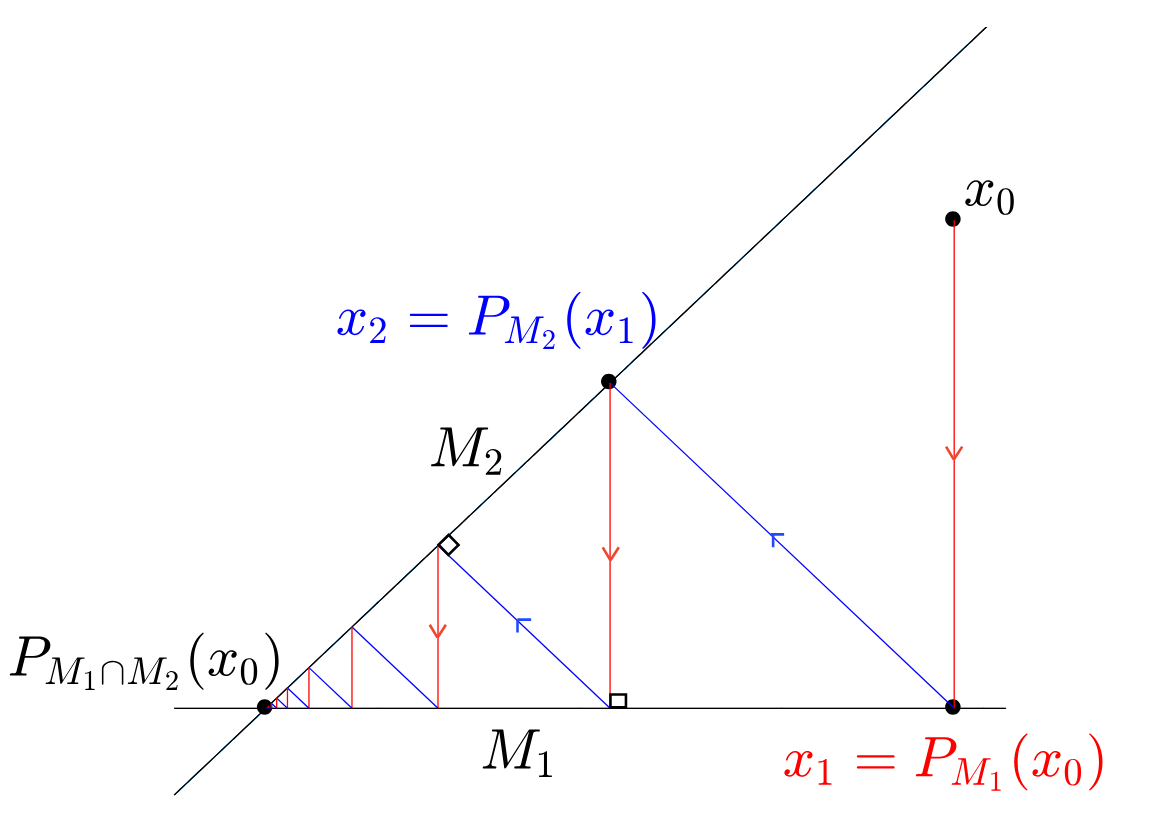
\includegraphics[width=0.5\linewidth]{images/convergence alternating projection.png}
        \caption{from https://arxiv.org/pdf/1809.05858}
        \label{fig:placeholder}
    \end{figure}
    \item \textbf{Alternating Projection}
    The most primitive and intuitive approuch to solve these problems is by alternating projecting the point on the both sets.
    \begin{equation}
        x_{n+1} = P_BP_Ax_n
    \end{equation}
    We can visualise this to get an intuitive view as to why this converges.

    \item \textbf{ADMM}
    \item \textbf{Douglass rachford}
    the douglass rachford algorithm uses reflections instead of projection to achieve convergence.
    \begin{equation}
        x_{n+1} =\frac{1}{2}(I + R_BR_A)x_n
    \end{equation}
    Both alternating projection and douglass rachford are special cases of the same algorithm, if we define the relaxed reflection / projection as 
    \begin{equation}
    \begin{split}
        R_C^{\gamma}(x) &= (2 - \gamma)(P_C - \mathrm{Id}) + \mathrm{Id}\\
        x_{n+1} &= (\lambda I + (\lambda-1)R_B^\gamma R_A^\gamma )x_n\\
    \end{split}
    \end{equation}
    {https://arxiv.org/pdf/1809.07181}\\
    When $\gamma$ goes to 1 the  and lambda goes to zero, we get the original alternating projections approuch 
    TODO:dit nalezen.
    \begin{figure}
        \centering
        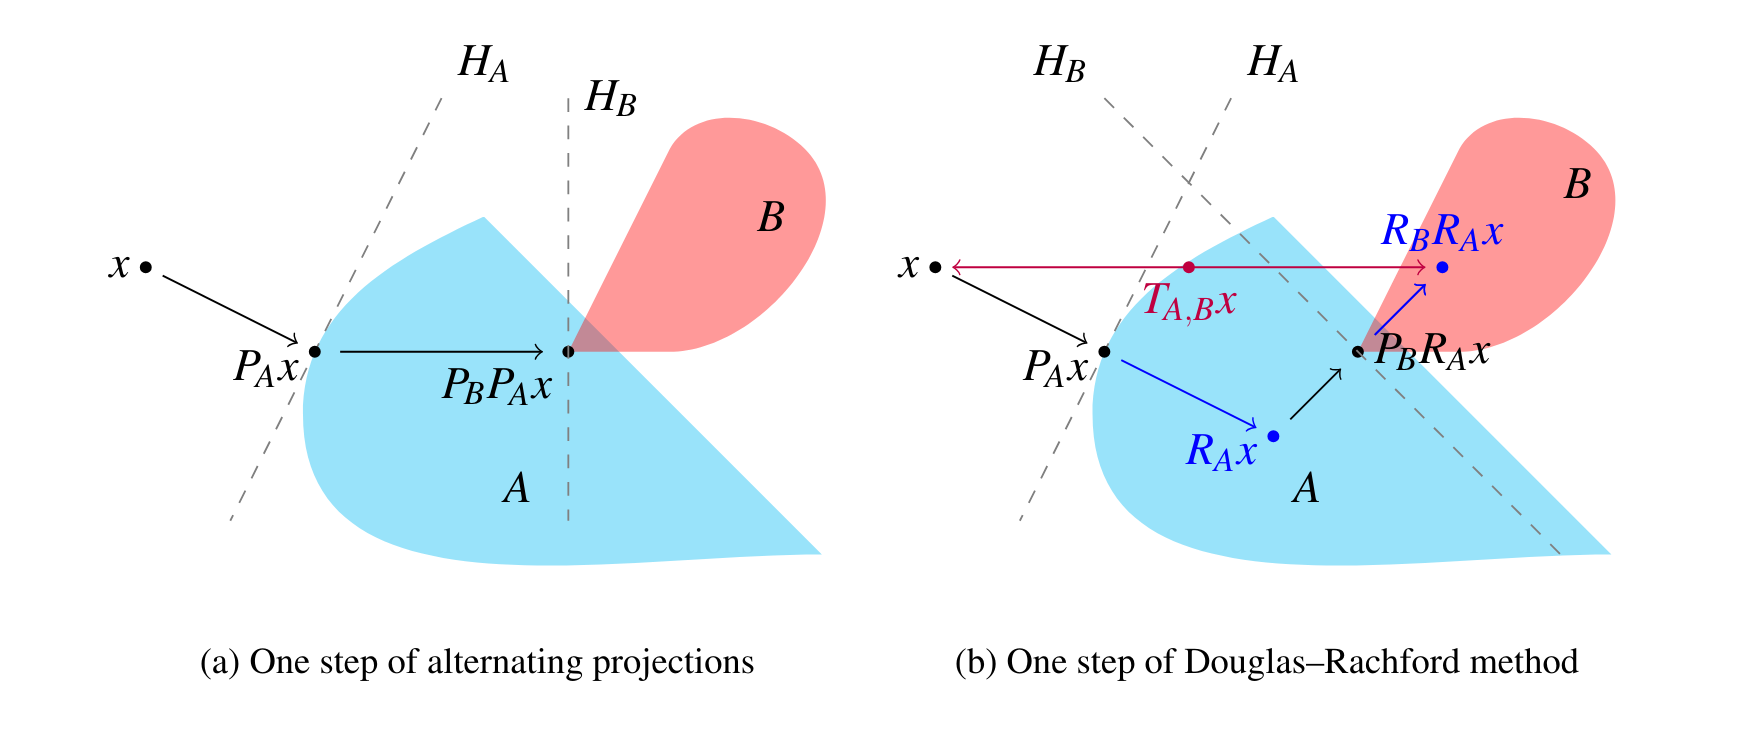
\includegraphics[width=0.5\linewidth]{images/douglas rachford.png}
        \caption{from https://arxiv.org/pdf/1809.07181}
        \label{fig:placeholder}
    \end{figure}
    \item \textbf{ideas to test}
    \begin{itemize}
        \item acceleration, 
    \begin{figure}
        \centering
        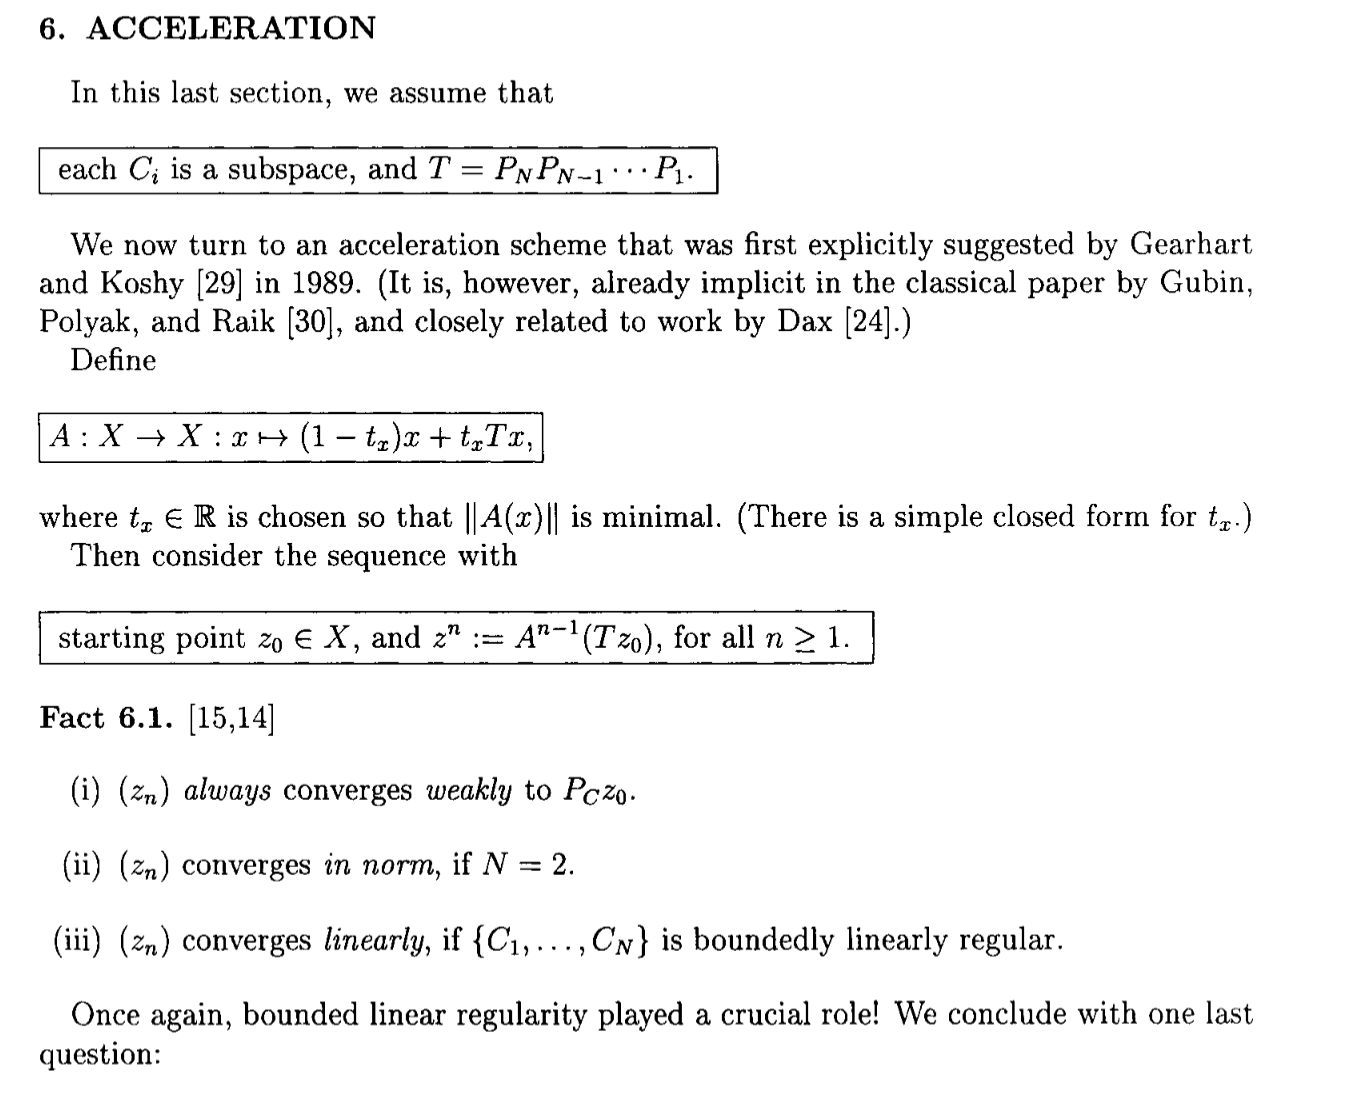
\includegraphics[width=0.5\linewidth]{image.png}
        \caption{Projection Algorithms: Results and Open Problems
}
        \label{fig:placeholder}
    \end{figure}
    
    \end{itemize}
    \end{itemize}

    \subsection{Reproduction experiments}
    In this section a reproduction of a subset of the experiments in relevant literature is performed.
    \subsubsection{NMF}
    An interesting use case of the 
    \subsubsection{classifier}
    \subsubsection{notes on diffusion neural networks}
    Basic idea diffusion probabilistic models, are parametrized Markov chains who produce smaples representing the training data after a finitie number of time. The task of the model is to predct the transitions of this chain, which represent a reverse diffusion process.
    Mathematically speaking it represents the flowing model.
    $X_0$ start with a normal distribution with both $\mathbf{N}(0,I)$. And then each subsequent transition is defined as $p(x_{t-1}|x_t) =\mathbf{N}{(x_{t-1}};\mu_\theta{(x_t,t)},\sigma_\theta{(x_t,t)}) $
    ..TODO copy forward process.

    Training is performed by minimizing the MSE between the added noise and the noise that the model predicts will be added 
    $L := E_{t, x_0, \epsilon} \left[ ||\epsilon - \delta_\theta(\sqrt{\bar{\alpha}_t} x_0 + \sqrt{1 - \bar{\alpha}_t} \epsilon, t)||^2 \right]   $
    All of this is compatible with pjax without needing any modifications  adding new projection operators.
    
    

